\subsection{Initial Graphics Exchange Specification (IGES) file}
\label{lr_sec:IGES}
% what is IGES
% why IGES
\paragraph{}
The Initial Graphics Exchange Specification (IGES) is one of the standard file formats that allows the digital data exchange among the CAD industries, proposed by the United States Air Force (USAF) Integrated Computer Aided Manufacturing (ICAM) project \citep{uspro2006}.
The initial propose of the ICAM was to significantly decrease the expenditure of data exchange in Aerospace manufacturing industry by developing procedures processes and CAD softwares.
In order to minimize the gap between parts design and manufacturing in Aerospace industry, ICAM planed to improve the CAD software so that it can produce the numerical control programs automatically for the complex Computer Numerically Controlled (CNC) machine tools.
One of the significant problem of it is that the data structure of the output of different CAD softwares can be different between each others.
Later, this problem was solved by the introduction of the IGES.
% development
\paragraph{}
The IGES had not gain popularity until 1988, when United State Department of Defense (USDoD) accepted the IGES file only for the contract of all weapons system if the products are delivered in digital form.
Consequently, any CAD software whose targeting customers want to sell their products to USDoD must support this file specification in terms of reading and writing.


% In the proposed approach, the geometry will be imported from the IGES file.
% IGES file can be easily exported from almost all popular CAD softwares such as AutoCAD.
% In this section, we give a brief overview of IGES file format.
% For more detailed description and implementation aspects, interested readers can refer to \citep{uspro2006}.
% data structure
% \subsubsection{General data structure}
\paragraph{}
A typical IGES file will be divided into 5 sections: start section, global section, directory entry section, parameter data section and terminate section as shown in Fig.~\ref{lr_fig:iges_data_form}.
The mathematical tool that represents most of geometric shapes in the IGES file is the NURBS curve in 2D and the NURBS surface in 3D which will be introduced in Sec.~\ref{lr_sec:NURBS}
% \paragraph{Start section}
% The start section provides a human-readable description about the file.
% This section shall always have the letter `S' in 73rd column.
% Data field of the start section will start at column 1 and end at column 72.
% The field can contain any text message expect ASCII control characters.
% Start section must appear in the file.
% The text can be empty but the sequence field shall not left empty.

% \paragraph{Global section}
% The global section describe the preprocessor and information that are necessary to handle the file by post-processors.
% Similar to start section, global section will always have the letter `G' in 73rd column.
% Parameters for the global section will be discussed later.
%
\begin{figure}[!ht]
    \centering
    \scalebox{0.4}{
        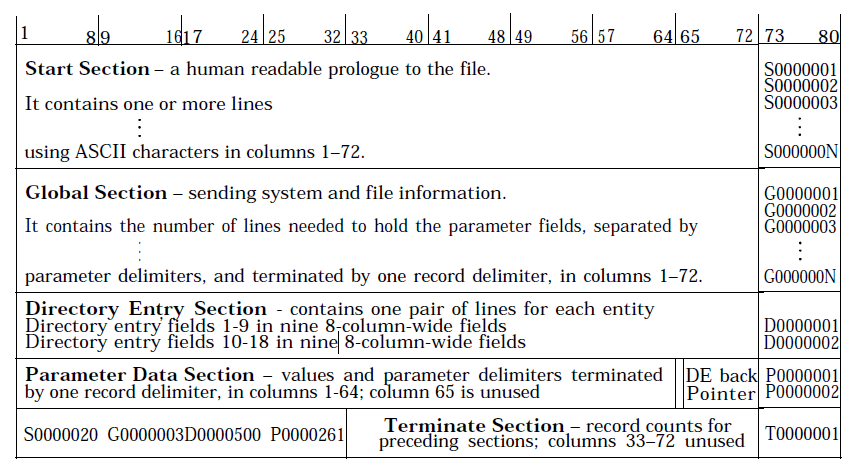
\includegraphics{literature/images/lr_iges_data_form.png}
    }
    \caption{File structure of an IGES file}
    \label{lr_fig:iges_data_form}
\end{figure}

\paragraph{}
